

\chapter{Estado del arte}

\lettrine{S}{on} muchos los estudios que se han publicado acerca del tema de la minería de opiniones. En esta investigación nos centraremos las técnicas más comunes de aprendizaje supervisado analizando distintos métodos tanto de clasificación como de preprocesamiento del texto.

En este capítulo describiremos el estado actual de los modelos de clasificación.

\section{Clasificación}
En términos de clasificación de sentimientos son muchos los trabajos publicados en los últimos tiempos (ver fig. \ref{pubsent}) debido a, como ya hemos comentado, el auge de las redes sociales y de la necesidad de las empresas por realizar estudios de mercado y de satisfacción de sus clientes.

\begin{figure}[!ht]
	\centering
	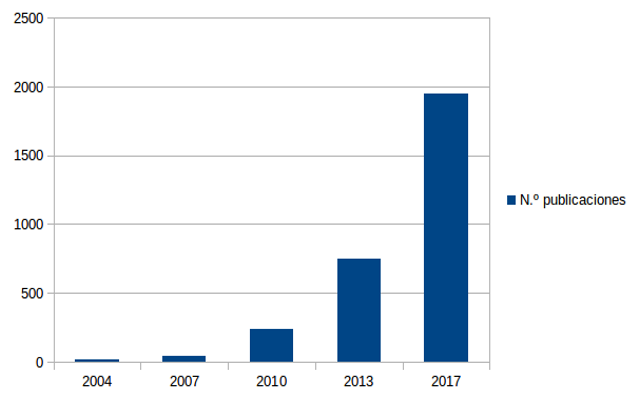
\includegraphics[width=0.75\textwidth]{imaxes/pubsentAnalisis.png}
	\caption{Publicaciones sobre Análisis de sentimientos en el IEEE desde 2004 hasta la actualidad}
		\label{pubsent}
\end{figure}

Dada la amplia extensión de métodos utilizados\footnote{http://www.sciencedirect.com/science/article/pii/S2090447914000550} para resolver este problema nosotros nos centraremos en la aproximación que utiliza algoritmos de aprendizaje automático, basándose la mayoría de estos estudios en los trabajos de Pang et al. \cite{Pang} intentando diseñar métodos más efectivos de extracción de características para mejorar la clasificación. En este último campo podríamos realizar una subdivisión atendiendo al tipo de algoritmo utilizado:

\begin{itemize}
	\item Machine Learning: Algoritmos tradicionales de aprendizaje supervisado, en los que se pretende obtener una matriz de características que servirán para extraer patrones que dividan los textos en distintas clases.
	\item Deep Learning: Se trata de algoritmos más novedosos, que están obteniendo alta relevancia en los últimos años (fig. \ref{pdeep}) gracias a la mejora de la capacidad de procesamiento de las GPU actuales. Estos modelos nos permiten obtener unos resultados mejores que los modelos tradicionales y además se ejecutan de forma más rápida gracias al alto rendimiento de las GPUs. 
	
	Además mediante esta rama de clasificación el vector de características se compone de Word Embeddings (WE) los cuales son mucho más ricos en información relacionada con la palabra que las features utilizadas en algoritmos tradicionales, ya que capturan información sobre similitud y características semánticas de las palabras.
	
	\begin{figure}[!ht]
		\centering
		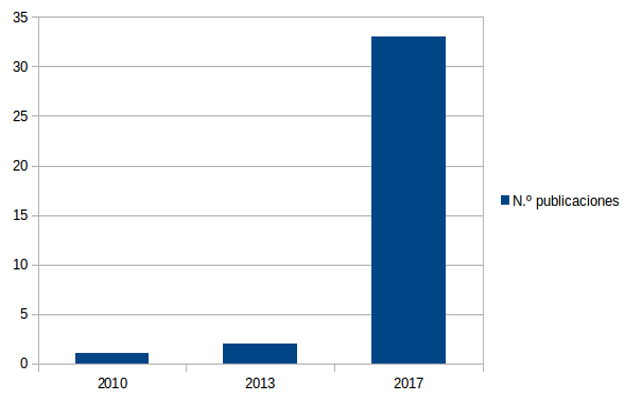
\includegraphics[width=0.75\textwidth]{imaxes/pubsDeep.png}
		\caption{Publicaciones en el IEEE desde 2010 que están relacionadas al término de búsqueda: sentiment analysis deep learning.}
				\label{pdeep}
	\end{figure}
\end{itemize}
Destacamos en esta sección los estudios realizados en la Universidad de Stanford \cite{Stanford}, obteniendo una precisión del 85.4\% para predicción binaria a nivel de oración.

\section {Conclusión}

Vistos los estudios anteriormente citados, vamos a realizar una implementación utilizando algoritmos típicos de Machine Learning que nos sirva como línea base, para posteriormente procurar mejorarla, tanto mejorando los procesos de tratamiento del texto como implementando modelos de Deep Learning.